\section{Arquitectura embebida}

\subsection{La política que corre a bordo}

La mochila deja que el insecto explore solo y estimula lo mínimo. La política es una máquina
de ocho estados que avanza una vez por cuadro térmico, diez veces por segundo
(figura~\ref{fig:fsm}). Usa tres entradas: cuántos píxeles calientes hay y de qué lado, si el
insecto está quieto según la IMU, y un número al azar.

\begin{figure}[H]
\centering
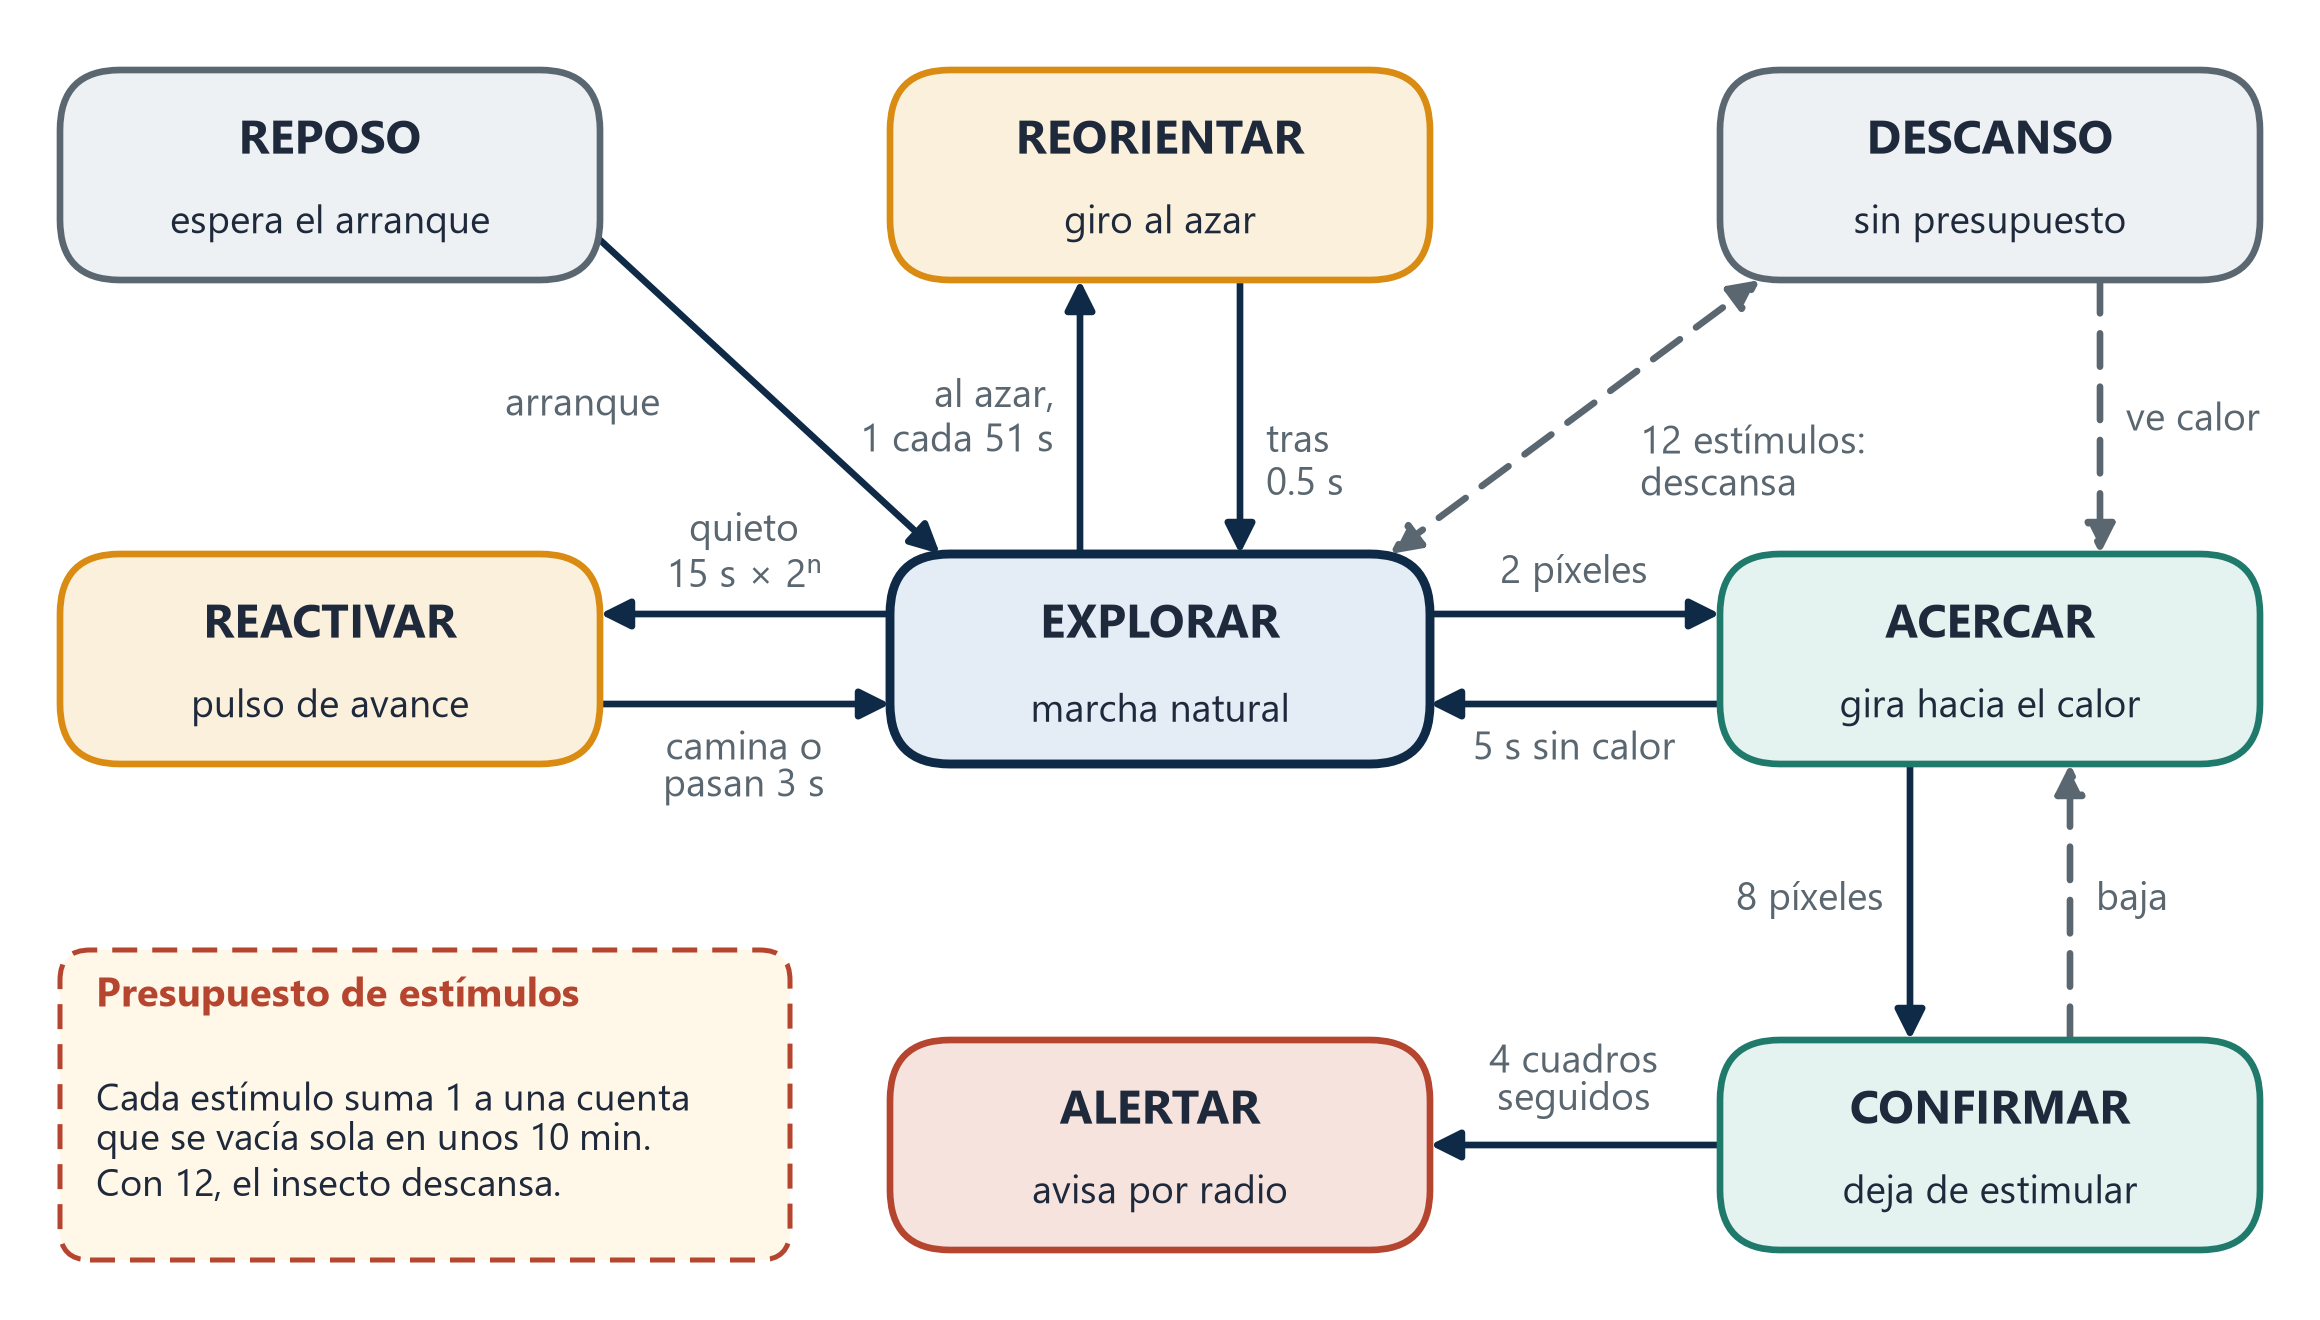
\includegraphics[width=0.86\textwidth]{figs/fsm_politica.png}
\caption{Máquina de estados de la política. Las flechas punteadas no producen estímulo.}
\label{fig:fsm}
\end{figure}

Tres reglas la distinguen de un control remoto:
\begin{itemize}
  \item \textbf{Espera que se duplica.} Si el insecto lleva 15~s quieto recibe un pulso de avance. Si
        en 3~s no arranca, la siguiente espera es de 30~s, luego 60 y 120. Un insecto que no responde
        deja de recibir estímulos inútiles.
  \item \textbf{Giros al azar.} En promedio cada 51~s, un giro a un lado elegido al azar. Es lo que
        despega al insecto de la pared que venía siguiendo~\cite{dirafzoon2017}.
  \item \textbf{Presupuesto de estímulos.} Cada estímulo suma 1 a una cuenta que pierde $1/256$ de su
        valor cada 2.3~s, con lo que se vacía con una constante de unos 590~s, cercana a la recuperación
        del insecto. Con 12 acumulados la mochila deja de estimular. Así acota la habituación y la
        carga sobre el animal sin tener que medir su respuesta.
\end{itemize}

\subsection{El núcleo digital}

\begin{figure}[H]
\centering
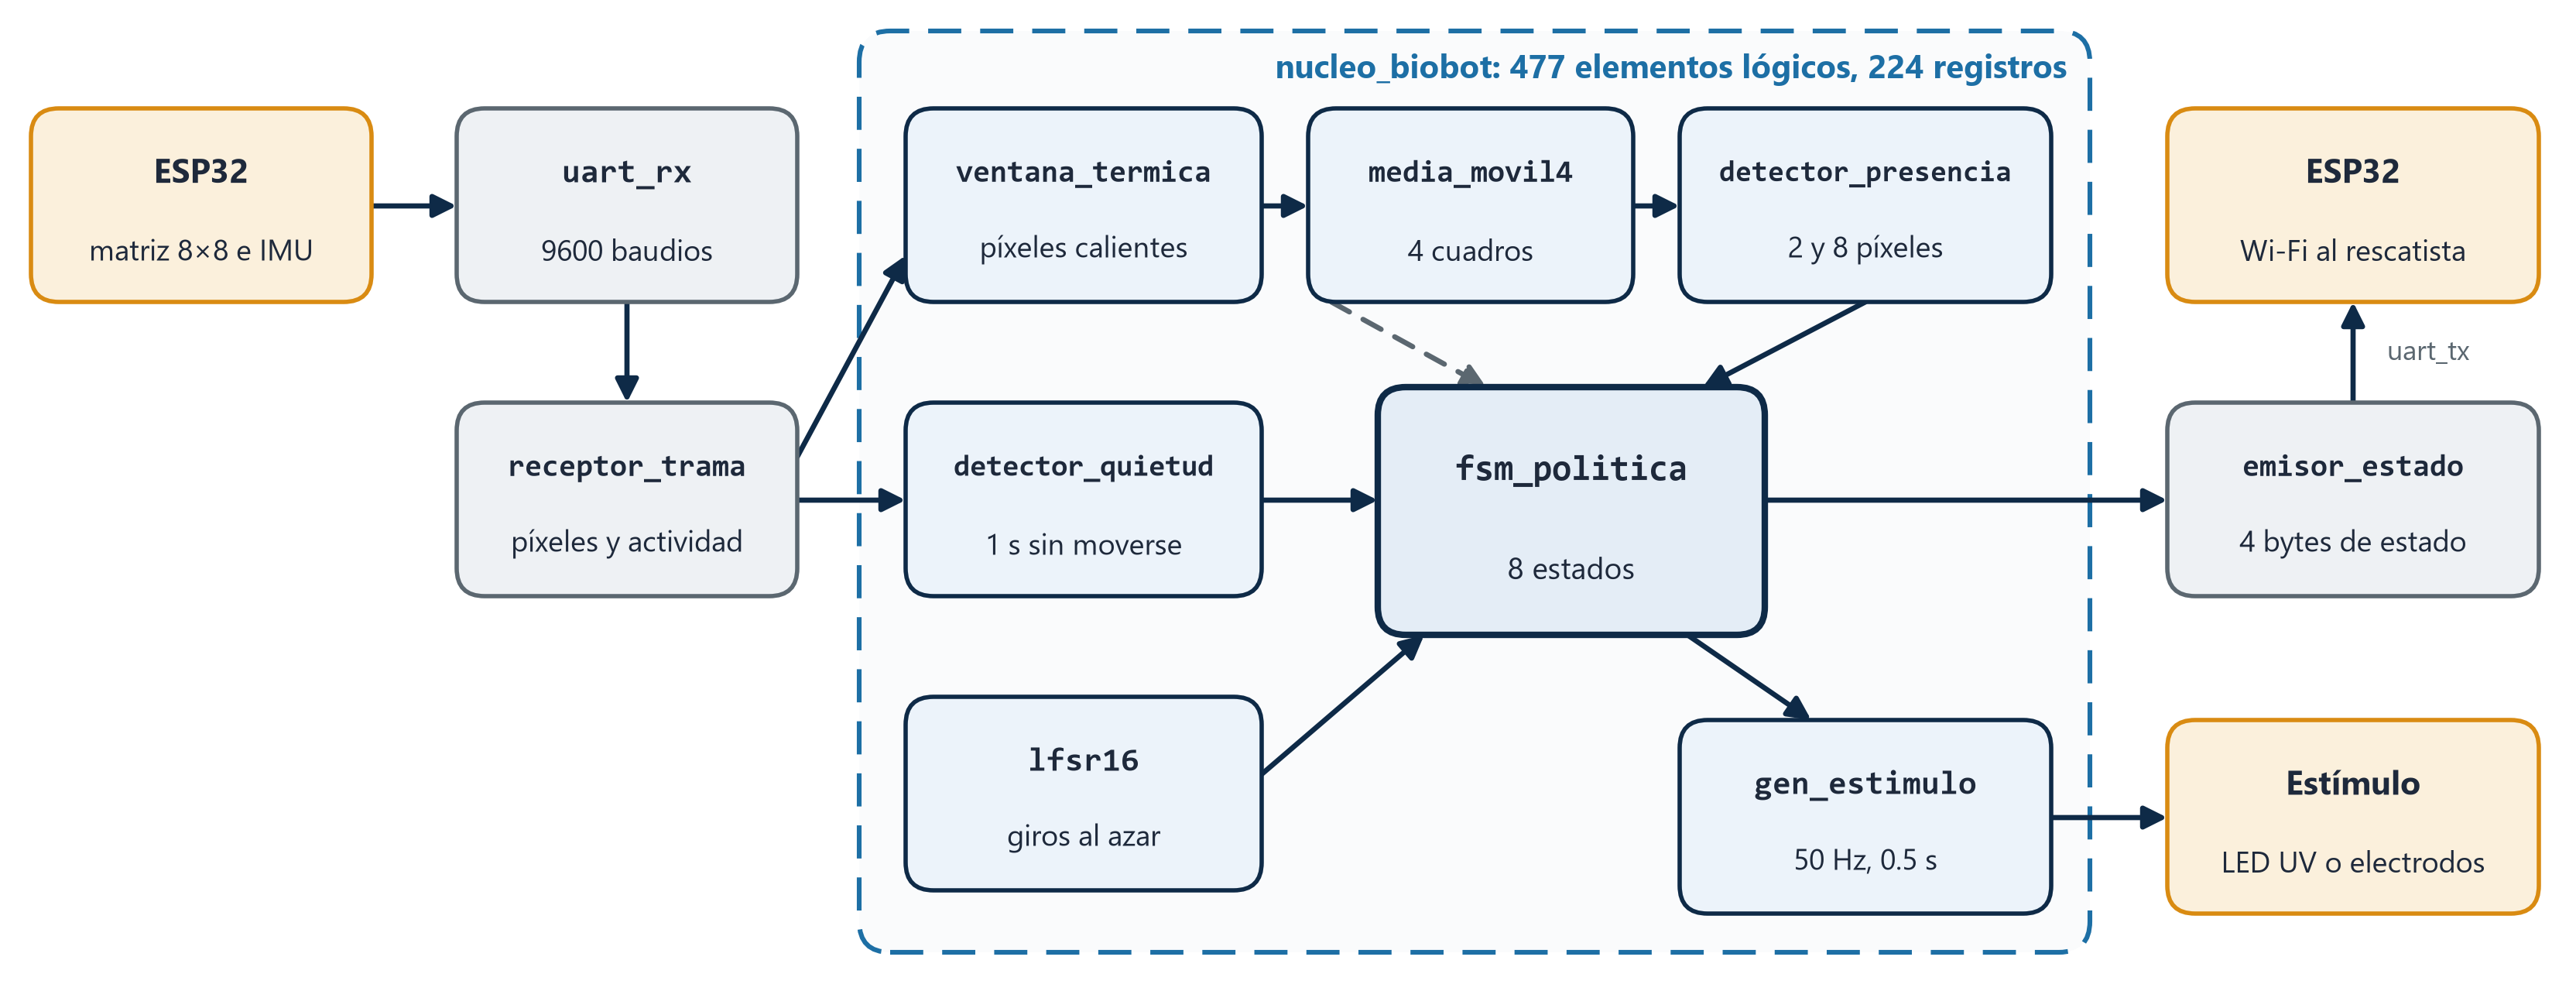
\includegraphics[width=\textwidth]{figs/nucleo_digital.png}
\caption{Módulos Verilog del prototipo. Lo que queda dentro del recuadro punteado es lo que iría en el
chip; lo de fuera es el enlace serie con el ESP32, que en la mochila se sustituye por el lector del
sensor y por la radio.}
\label{fig:nucleo}
\end{figure}

\begin{table}[H]
\centering\footnotesize
\caption{Módulos del núcleo y recursos tras la síntesis en Quartus Prime 24.1 para el
\sig{10M50DAF484C7G}.}
\label{tab:modulos}
\rowcolors{2}{SoftGray}{white}
\begin{tabularx}{\textwidth}{@{}>{\ttfamily\raggedright\arraybackslash}p{3.3cm} >{\raggedright\arraybackslash}X r r@{}}
\toprule
\rowcolor{TableHead} \normalfont\textbf{Módulo} & \textbf{Función} & \textbf{Elem. lógicos} & \textbf{Registros} \\
\midrule
ventana\_termica & Recibe el cuadro píxel por píxel; cuenta los calientes, dice de qué lado están y calcula la media del cuadro & 160 & 61 \\
media\_movil4 & Promedia los últimos cuatro conteos para quitar el vaivén de la marcha & 40 & 28 \\
detector\_presencia & Compara con 2 y con 8 píxeles y exige cuatro cuadros seguidos & 9 & 4 \\
detector\_quietud & Declara quieto al insecto tras 1~s sin actividad en la IMU & 10 & 4 \\
lfsr16 & Números seudoaleatorios para los giros & 16 & 16 \\
fsm\_politica & Los ocho estados, la espera que se duplica y el presupuesto de estímulos & 181 & 64 \\
gen\_estimulo & Tren bifásico de 50~Hz y 0.5~s por el canal pedido & 64 & 47 \\
\midrule
\normalfont\textbf{Núcleo} & & \textbf{477} & \textbf{224} \\
\normalfont Enlace serie y displays & \sig{uart\_rx}, \sig{uart\_tx}, \sig{receptor\_trama}, \sig{emisor\_estado} y decodificadores & 245 & 148 \\
\midrule
\normalfont\textbf{Prototipo completo} & 43 pines, $f_{\max}=72.08$~MHz, holgura de 6.13~ns a 50~MHz & \textbf{722} & \textbf{372} \\
\bottomrule
\end{tabularx}
\end{table}

\subsection{Verificación}

Antes de escribir el Verilog se programó un modelo de referencia en Python que hace las mismas
cuentas con enteros, registro por registro. Ese modelo genera los cuadros de prueba y la
respuesta esperada; los bancos de prueba comparan cuadro por cuadro.

\begin{table}[H]
\centering\footnotesize
\caption{Resultados de simulación con Icarus Verilog 12.}
\label{tab:bancos}
\rowcolors{2}{SoftGray}{white}
\begin{tabularx}{\textwidth}{@{}>{\ttfamily\raggedright\arraybackslash}p{2.8cm} >{\raggedright\arraybackslash}X >{\raggedright\arraybackslash}p{4.4cm}@{}}
\toprule
\rowcolor{TableHead} \normalfont\textbf{Banco} & \textbf{Qué prueba} & \textbf{Resultado} \\
\midrule
tb\_nucleo & 11\,424 cuadros: exploración con pausas, insecto que no responde, acercamiento y detección, ambiente a 30 y 37.5~\textdegree C, objeto a 47.5~\textdegree C y 3\,000 cuadros al azar & 11\,424 de 11\,424 coinciden; se visitan los ocho estados \\
tb\_gen\_estimulo & Periodo, ciclo de trabajo, duración, fases sin traslape y disparo a medio tren & 3 de 3 trenes: 25 periodos de 20.000~ms, 500.0~ms \\
tb\_top & Sistema completo por UART: 500 cuadros hasta la detección confirmada & 500 de 500 respuestas coinciden \\
tb\_demo & Núcleo e insecto de prueba en el mismo chip: persona, sin persona, objeto caliente e insecto que no responde & 4 de 4: solo alerta con persona, en el cuadro 558 \\
tb\_dos\_tarjetas & Dos tarjetas unidas solo por las dos líneas de UART: persona y objeto caliente & 2 de 2: alerta en el cuadro 557; sin alerta con el objeto \\
\bottomrule
\end{tabularx}
\end{table}

El escenario de ambiente tibio confirma el criterio doble de la sección~\ref{sec:deteccion}: con todo el cuadro a
30~\textdegree C no hay píxeles calientes, un objeto a 47.5~\textdegree C no cuenta, y una mancha a
34.5~\textdegree C sí. Con el ambiente a 37.5~\textdegree C la mancha desaparece, que es el límite físico
ya descrito.

\subsection{Camino a un chip propio}

El núcleo usa 224 registros y unos 450 bloques combinacionales. En la biblioteca de alta densidad
de SKY130, un registro ocupa 20.0~$\mu$m$^2$ y una compuerta NAND de dos entradas
3.75~$\mu$m$^2$~\cite{skywater}. Con unos 6~$\mu$m$^2$ por celda combinacional y 50~\% de
utilización, el área estimada es
\begin{equation}
\frac{224\times20.0+450\times6}{0.5}\approx14\,400~\mu\text{m}^2=0.014~\text{mm}^2 ,
\end{equation}
es decir, un módulo de Tiny Tapeout ($160\times100~\mu$m) o dos~\cite{tinytapeout}. Es una
estimación por conteo: el número real saldrá del flujo de SKY130 en la máquina virtual del curso.
Las corridas abiertas cierran el 30 de noviembre de 2026 y entregan chips a mediados de 2027.
Mientras tanto, una iCE40 UltraLite de 1\,248 LUT y 2~mg aloja el núcleo con holgura.

\subsection{Prototipo y demostración}

\begin{figure}[H]
\centering
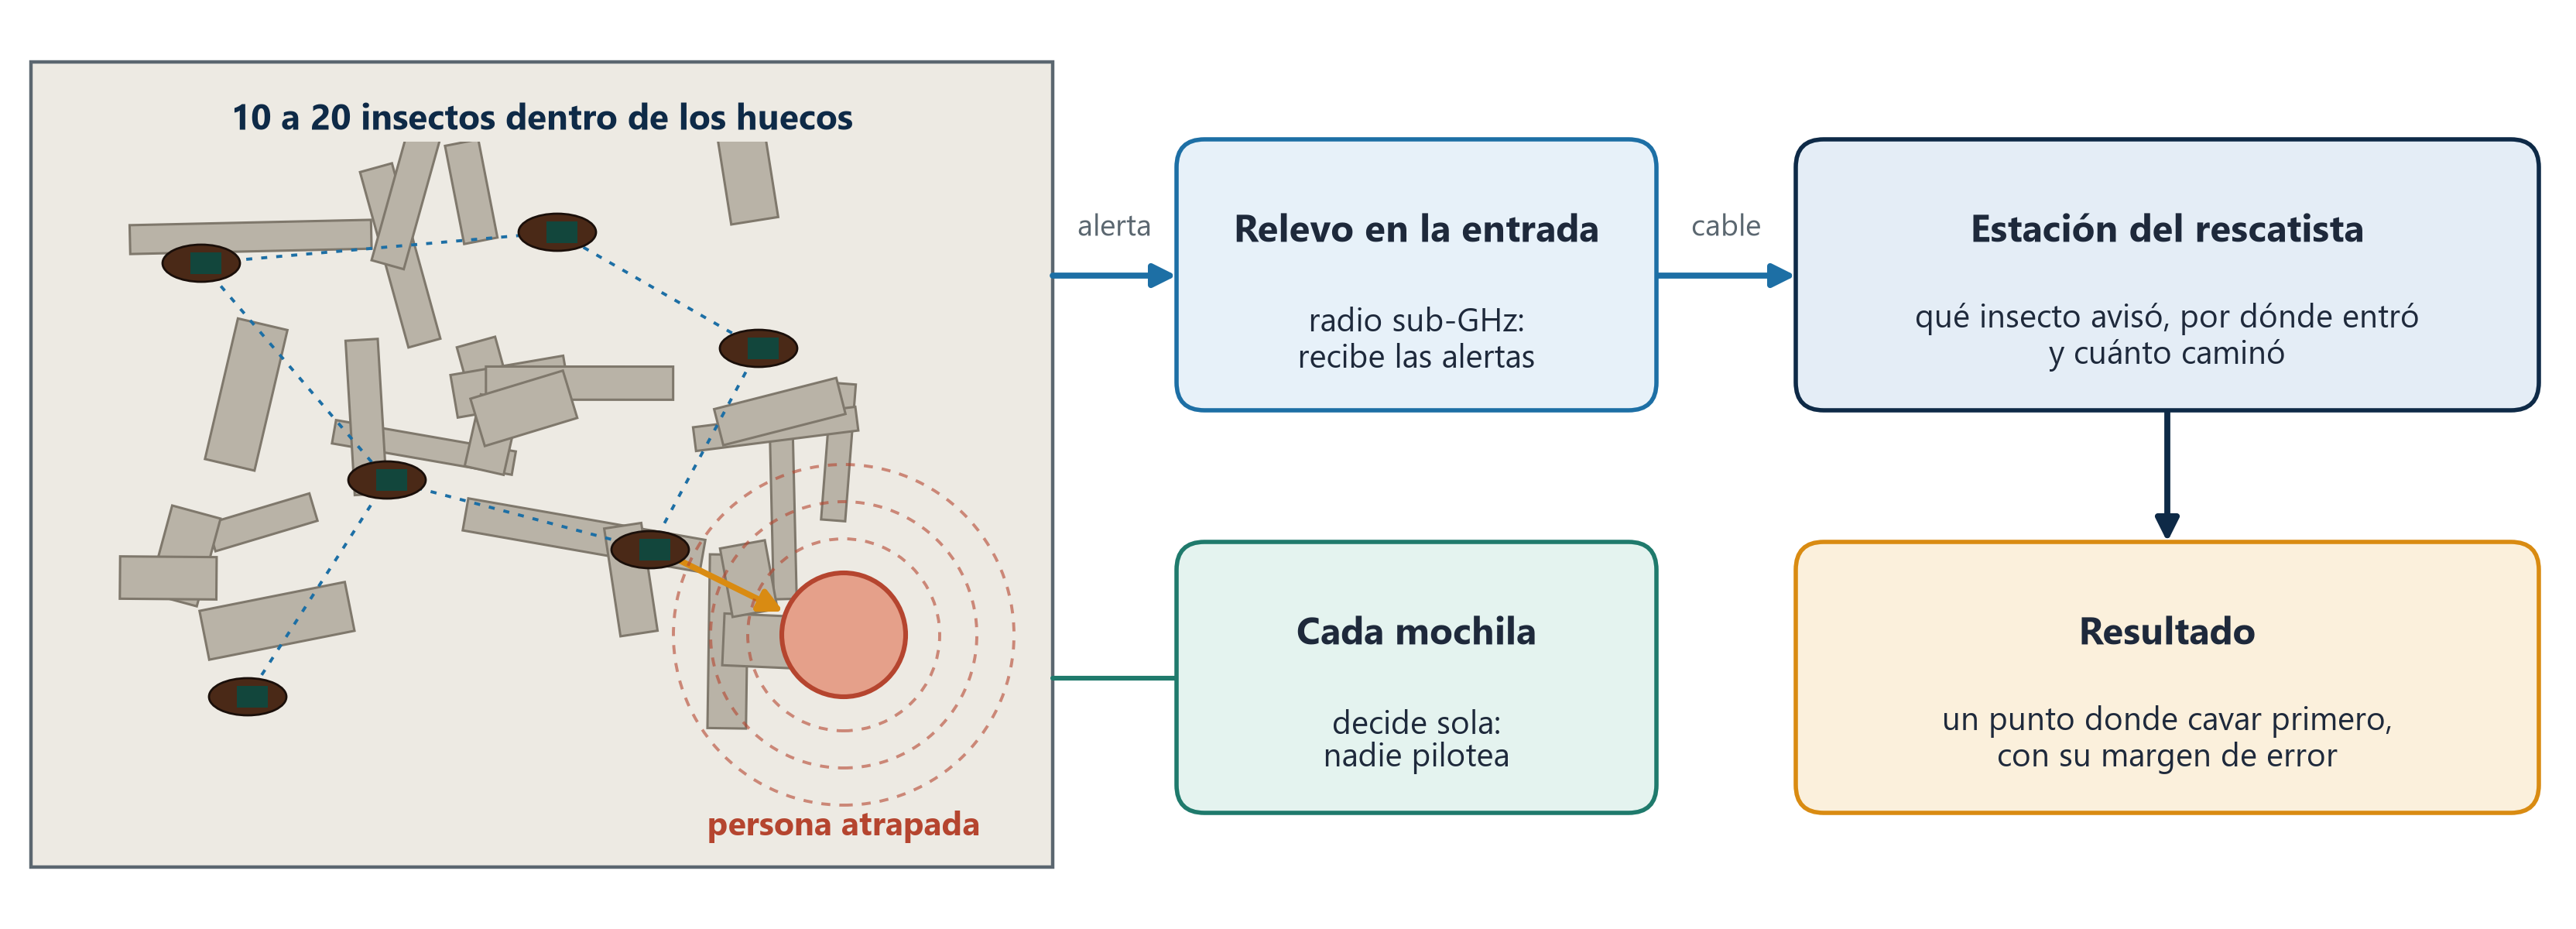
\includegraphics[width=\textwidth]{figs/sistema.png}
\caption{Sistema completo: del enjambre al rescatista.}
\label{fig:sistema}
\end{figure}

En el prototipo, el ESP32 lee la matriz térmica y manda cada cuadro por UART a la DE10-Lite
(66 bytes: encabezado, actividad y 64 píxeles); la tarjeta corre el núcleo y contesta con cuatro
bytes de estado.

\textbf{Prueba en dos tarjetas reales.} Mientras llega el sensor, una segunda DE10-Lite hace de
insecto y de matriz térmica. Calcula los 64 píxeles que vería la mochila según la distancia y el
rumbo, los manda a 9\,600 baudios y mueve a un insecto de prueba según los estímulos que recibe.
Las unen tres cables: dos líneas de UART cruzadas y tierra. El 11 de noviembre de 2026 se corrieron
los cuatro escenarios; los LED y los displays se leyeron por el cable USB con una sonda de Quartus.

\begin{table}[H]
\centering\footnotesize
\caption{Los cuatro escenarios en dos DE10-Lite reales, en tiempo real.}
\label{tab:tarjetas}
\rowcolors{2}{SoftGray}{white}
\begin{tabularx}{\textwidth}{@{}>{\bfseries\raggedright\arraybackslash}p{3.2cm} >{\raggedright\arraybackslash}X >{\raggedright\arraybackslash}p{3.6cm}@{}}
\toprule
\rowcolor{TableHead} Escenario & Lo medido en las tarjetas & Simulación \\
\midrule
Persona a 1.65~m & Acercar a los 26.3~s con 2 píxeles; 8 píxeles a los 54.6~s; alerta a los 55.1~s, cuatro cuadros después; la otra tarjeta recibe la alerta & Alerta a los 55.6~s \\
Objeto a 47.5~\textdegree C & Ningún píxel caliente, ni a 0.2~m; sin alerta en 45~s & Sin alerta \\
Sin persona & Un pulso de avance cuando el insecto se detuvo; sin alerta en 75~s & Sin alerta \\
Insecto que no responde & Reactivar a los 16 y a los 49~s; sin alerta en 75~s & Reactivar a los 16 y a los 49~s \\
\bottomrule
\end{tabularx}
\end{table}

El circuito de la mochila es el mismo que se usará con el ESP32 y el sensor: no se le cambia nada.
El insecto de prueba no es el modelo de marcha de la simulación de misiones; es un banco con
valores redondos que solo sirve para cerrar el lazo. Faltan dos pruebas:
\begin{itemize}
  \item \textbf{Con una persona real.} La matriz apunta a la mesa; al acercar una mano, los LED de
        la tarjeta muestran el paso de explorar a acercar, confirmar y alertar, y el display muestra
        los píxeles calientes.
  \item \textbf{Con un insecto simulado.} La computadora corre la simulación de misión y le manda
        a la tarjeta lo que vería y sentiría la mochila; la tarjeta devuelve los estímulos y la simulación
        mueve al insecto. Es el circuito real dentro del lazo, sin usar animales.
\end{itemize}
